\documentclass{llncs}
\usepackage[T1]{fontenc}
\usepackage{lmodern}
\usepackage{hyperref}
\usepackage{cite} % Multiple citations in one \cite command
\usepackage{pgfplotstable}
\usepackage{array} % Required for pgfplotstable dec sep align
\pgfplotsset{compat=1.12}
\usepackage{booktabs}

\usepackage{enumitem}
\setlist{parsep=0pt, listparindent=0.5cm}

\begin{document}
\title{A Comparison of Parallel Graph Processing Benchmarks}
\author{Samuel D. Pollard \and Boyana Norris}
\institute{University of Oregon \\
	Eugene OR 97403, USA \\
	\email{\{spollard,norris\}@cs.uoregon.edu}
}
\maketitle
\begin{abstract}
The increasing popularity of large network analysis problems has led to the emergence of many parallel and distributed graph processing systems---one survey in 2014 identified over 80. Since then, the landscape has evolved; some packages have become inactive while more are being developed. Determining the best approach for a given problem is infeasible for most developers. To enable easy, rigorous, and repeatable comparison of the capabilities of such systems, we present an approach and associated software for analyzing the performance and scalability of parallel, open-source graph processing systems. We demonstrate our approach on five graph frameworks: GraphMat, the Graph500, the Graph Algorithm Platform, GraphBIG, and PowerGraph using synthetic and real-world datasets. We examine previously overlooked aspects of parallel graph processing performance such as phases of execution and energy usage for three algorithms: breadth first search, single source shortest paths, and PageRank and compare our results to Graphalytics.
\end{abstract}

\section{Introduction and Related Work}

Our research is motivated by the current state of parallel graph processing. The most comprehensive survey, released in 2014, identified and taxonomized over 80 different parallel graph processing systems without including domain specific languages \cite{Doekemeijer:2015:GPFSurvey}. The systems described operate with a wide range of parallelism paradigms and target architectures such as GPU \cite{Zhong:2014:Medusa, Kang:2009:Pegasus}, shared memory CPU \cite{Shun:2013:Ligra, kyrola:2012:Graphchi, Nguyen:2013:Galois}, a combination of CPU and GPU \cite{Gharaibeh:2012:Totem}, distributed filesystem based approaches \cite{Xin:2013:GraphX}, and distributed memory with MPI \cite{Gregor:2005:PBGL}.

Beyond the systems described by Doekemeijer and Varbanescu, the problem has compounded with the addition of even more proprietary and open source projects such as \cite{Cheramangalath:2015:Falcon}, \cite{Perez:2015:Ringo}, distributed memory approaches such as \cite{Hong:2015:PGX}. domain-specific languages \cite{Hong:2012:GreenMarl}, distributed database querying, \cite{Rodriguez:2015:Gremlin}, as well as novel communication schemes \cite{Edmonds:2013:ActiveMessages}. At the outset, this plethora of choices makes the question, ``which system is the best for my problem?'' daunting.

In addition to libraries with associated APIs there has also been a propagation of ``reference implementations'' which implement the most common graph algorithms such as \cite{Beamer:2015:GAPBench, Nai:2015:Graphbig}. Thus, even selecting a standard and a benchmark over which to compare various implementations is nontrivial. To quote Andrew Tanenbaum, ``The nice thing about standards is that you have so many to choose from.''

Another issue among parallel graph processing systems is the lack of comprehensive comparisons. One possible reason is the considerable effort involved in getting each system to run: satisfying dependencies and ensuring data are correctly formatted are generally nontrivial tasks. Beyond this, there are optimizations for each system which are not exploited in a na\"ive implementation. Addressing these issues helps provide an environment in which no graph processing system has an advantage.

Graphalytics \cite{Capota:2015:Graphalytics} also attempts to remedy these problems. However, in order for Graphalytics to analyze a graph processing system---Graphalytics calls these platforms---a programmer must implement Java classes as wrappers to call the particular implementations, satisfy dependencies, and set environment variables. These all require some knowledge of the inner workings of each system in addition to familiarity with the Graphalytics API.

The complexity of Graphalytics obfuscates the true behavior of the algorithm. We use GraphMat, the single source shortest paths algorithm, the dota-league dataset, and the default settings as an example here. By default, Graphalytics generates an HTML report giving the runtimes for each dataset in seconds. Two separate runs for a single dataset, all else being equal, gave 5.6 seconds. However, perusing the log files reveals a more complete picture: of these 5.6 seconds, 0.19 was spent computing the shortest paths while the remaining time consisted of building the necessary data structures.

With a plugin to Graphalytics called Granula \cite{Ngai:2015:Granula} one can explicitly specify a performance model to analyze specific execution behavior such as the amount of communication or runtime of particular kernels of execution. The requires in-depth knowledge of the source code and execution model which is not always available. Furthermore, creating such a model requires a high level of expertise with the given system and with Granula.

As with Graphalytics, the initial development effort is high but Granula paired with graphalytics allows automatic execution and compilation of performance results\footnote{An example of Granula can be seen at \url{https://github.com/tudelft-atlarge/graphalytics-platforms-graphx/tree/master/granula-model-graphx}}. Likewise, our approach provides automatic execution and performance analysis without requiring a performance and execution model for each system.

To showcase our methods we analyze the performance of several graph processing benchmarks to facilitate the selection among such systems. Our analysis is done with minimal source code modification.

\section{Experimental Setup}

\subsection{Graph Processing Systems}

This report explores four shared memory parallel graph processing platforms. The first three are so-called ``reference implementations'' while the fourth is included because it has been cited as highly performant \cite{Sundaram:2015:GraphMat}. Our target is shared memory CPU processing. Other popular libraries such as the Parallel Boost Graph Library \cite{Gregor:2005:PBGL} are not considered here because the authors do not provide reference implementations. The systems are:

\begin{enumerate}
	\item The Graph500\footnote{We used the most recent version from \url{https://github.com/graph500/graph500}, most similar to release 2.1.4.} \cite{Murphy:2010:Graph500}
	\item The Graph Algorithm Platform (GAP) Benchmark Suite \cite{Beamer:2015:GAPBench}
	\item GraphBIG \cite{Nai:2015:Graphbig}
	\item GraphMat \cite{Sundaram:2015:GraphMat}
\end{enumerate}

\subsection{Algorithms}

We consider three algorithms:

\begin{enumerate}
	\item Breadth First Search (BFS)
	\item Single Source Shortest Paths (SSSP)
	\item PageRank
\end{enumerate}

The canonical performance leaderboard for parallel graph processing is the Graph500 \cite{Murphy:2010:Graph500}. The advantage of the Graph500 is it provides standardized measurement specifications and dataset generation. The primary drawback with the Graph500 is it measures a single algorithm: breadth first search.

This report aims to add similar rigor to other graph algorithms by borrowing heavily from the Graph500 specification. The Graph500 Benchmark 1 (``Search'') is concerned with two kernels: the creation of a graph data structure from an edge list stored in RAM and the actual BFS\footnote{For a complete specification, see \url{http://graph500.org/specifications}}. We run the BFS using 32 random roots.

One straightforward extension to BFS and our second algorithm is the Single-Source Shortest Paths algorithm (SSSP). We use the same graph and the same source vertices as in BFS.

The third algorithm is PageRank. These three algorithms are used because of their popularity; most libraries provide reference implementations. All the experiments performed use the developer-provided implementations because we assume the vendor will provide a more performant implementation than us. While this limits the scope of the experiments it mitigates the bias inherent in any developer's programming skills.

\subsection{Machine Specifications}
Table~\ref{tab:specs} shows the specifications of the research machine. The disparity between the CPU's advertised clock speed and the ``CPU Clock'' row is a result of the Turbo Boost technology which can increase the clock speed to a limit. We use the manufacturer's published maximum clock speeds which can be found at \url{http://ark.intel.com}.

\begin{table}
	\centering
	% Keep in mind you can do this at the beginning: string replace={s1}{s2}
	% For arya I deleted Max RAM Freq	2133MHz
	\pgfplotstabletypeset[
	header=false,
	col sep=tab,
	string type,
	every head row/.style={output empty row, before row=\bottomrule},
	columns/0/.style={column type={|r|}},
	columns/1/.style={column type={l|}},
	every last row/.style={after row=\toprule},
	]{../report/specs.csv}
	\caption{The operating system is GNU/Linux version 4.4.0-22.}
	\label{tab:specs}
\end{table}

\subsection{Datasets}
We use the Graph500 synthetic graph generator which creates a Kronecker graph \cite{Leskovec:2010:Kronecker} with initial parameters of $A = 0.57, B = 0.19, C = 0.19,$ and $D = 1-(A+B+C) = 0.05$.

The Graphalytics results in Table~\ref{tab:graphalytics} were performed on the Dota-League dataset. This dataset contains 61,670 vertices and 50,870,313 edges. This dataset is sourced from the Game Trace Archive\cite{Guo:2012:GTA} and modified for Graphalytics\footnote{This dataset is available at \url{https://atlarge.ewi.tudelft.nl/graphalytics/}.}.

\section{Performance Analysis}

We use the Performance Application Programming Interface (PAPI) \cite{Browne:2000:PAPI} to gain access to Intel's Running Average Power Limit (RAPL), which provides access to a set of hardware counters measuring energy usage.


In Table~\ref{tab:graphalytics} we show the results from running Graphalytics. For an explanation of each algorithm used, see \cite{Iosup:2016:Graphalyticstech}.

From this we get only a broad overview of the two systems: GraphBIG and PowerGraph. In general, we see GraphBIG is more performant. However, results such as these are preliminary and do not show the complete picture.

[How to make this a paper worth submitting: add in PowerGraph as a platform and see how it fares using our method compared to Graphalytics. Also run this on different datasets and compare results.]

%\begin{table}[htb]
%	\centering
%	\begin{tabular}{l|c|c|c}
%		& BFS & SSSP & PR \\ \hline
%		Graph500 & & & \\ \hline
%		PBGL  & & & \\ \hline
%		GAP  & & & \\ \hline
%		GraphBIG  & & & \\ \hline
%		Galois  & & & \\ \hline
%		PowerGraph  & & &
%	\end{tabular}
%	\caption{Performance. Note that implementations of every algorithm are not availabe for every platform.}
%	\label{tab:reportcard}
%\end{table}

%Table~\ref{tab:perf} lists performance in milliseconds of runtime according to the graphalytics output. Graphalytics also outputs MTEPS or millions of traversed edges pers econd. However, the graphalytics version does not make sense in all cases: for example, computing the local clustering coefficient involves traversing each edge multiple times (proportional to the sparsity of the graph), while breadth first search (BFS) traverses each edge exactly once, and on na\:ive implementations single-source shortest paths (SSSP) may have $O(|E| + |V|^2)$ traversed edges.

\begin{table}
%	\begin{tabular}{l|r|r|}
%	 & PowerGraph & OpenG \\ \hline
%	BFS & 81.8 & 341 \\ \hline
%	SSSP & 1.64 & 15.0 \\ \hline
%	LCC & 54.6 & 142 \\ \hline
%	\end{tabular}
		\centering
		\pgfplotstabletypeset[
			col sep=comma,
			columns={[index]0,GraphBIG,PowerGraph},
			every head row/.style={after row=\midrule},
			columns/0/.style={string type, column type={l|}, column name={}},
			columns/openg/.style={dec sep align},
			columns/powergraph/.style={dec sep align}
		]{../report/runtime.csv}
	\caption{Performance results are in milliseconds. LCC is local clustering coefficient, PR is PageRank, CDLP is community detection using label propagation, and WCC is weakly connected components}
	\label{tab:graphalytics}
\end{table}


\begin{table}[!htb]
	\centering
	\begin{tabular}{l|c|c|c}
		System & Load Graph & \begin{tabular}[x]{@{}c@{}}Construct Data \\ Structure\end{tabular} & Run BFS \\ \hline
		Graph500 & 0.3474 & 0.3971 & 0.003380 \\
		GAP      & 2.351  & 0.1935 & 0.001393 \\
		GraphMat & 0.1511 & 1.101  & 0.1031 \\
		GraphBIG & 37.22  & N/A    & 0.1528 \\
	\end{tabular}
	\caption{The above table shows times for $2^{20}$ verties and the times are in seconds. The Graph500 generates the graph instead of loading it into a file. GraphBIG builds the graph and reads in the file simultaneously. These results were averaged across 32 roots.}
	\label{tab:fileload}
\end{table}

\begin{figure}
	\centering
	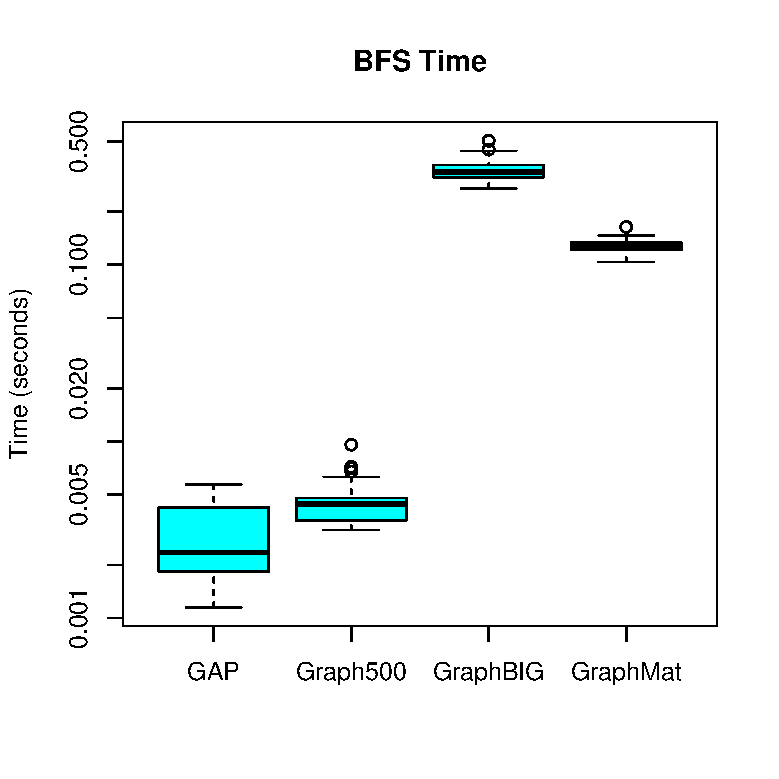
\includegraphics[width=0.6\columnwidth, trim=0 36pt 18pt 0, clip]{graphics/bfs_time.pdf}
	\caption{The $y$-axis is logarithmic.}
	\label{fig:bfs-time}
\end{figure}

\begin{figure}
	\centering
	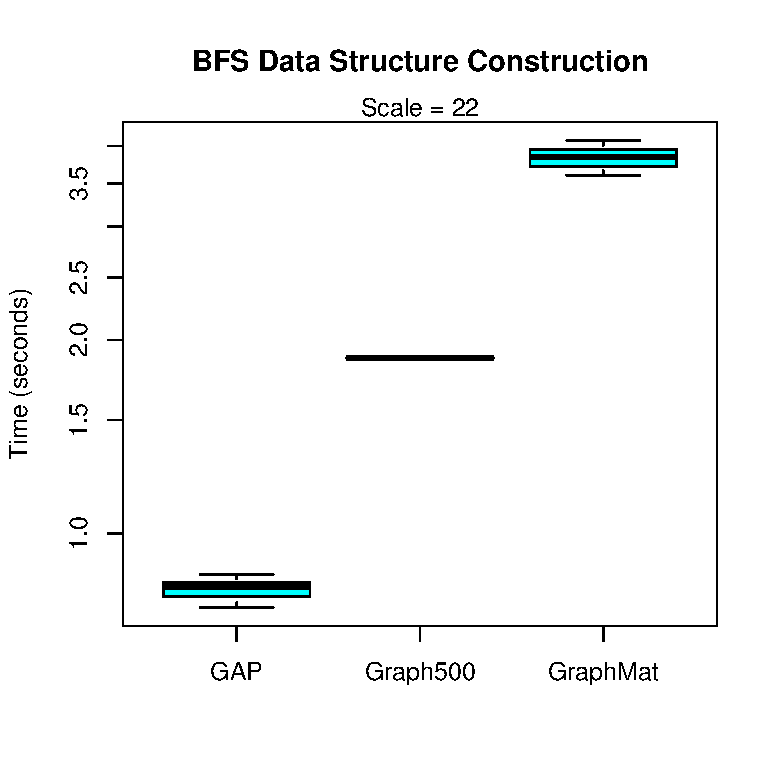
\includegraphics[width=0.6\columnwidth, trim=0 36pt 18pt 0, clip]{graphics/bfs_dsc.pdf}
	\caption{The $y$-axis is logarithmic. GraphBIG reads in the file and generates the data structure simultaneously so is omitted.}
	\label{fig:bfs-dsc}
\end{figure}

\begin{figure}
	\centering
	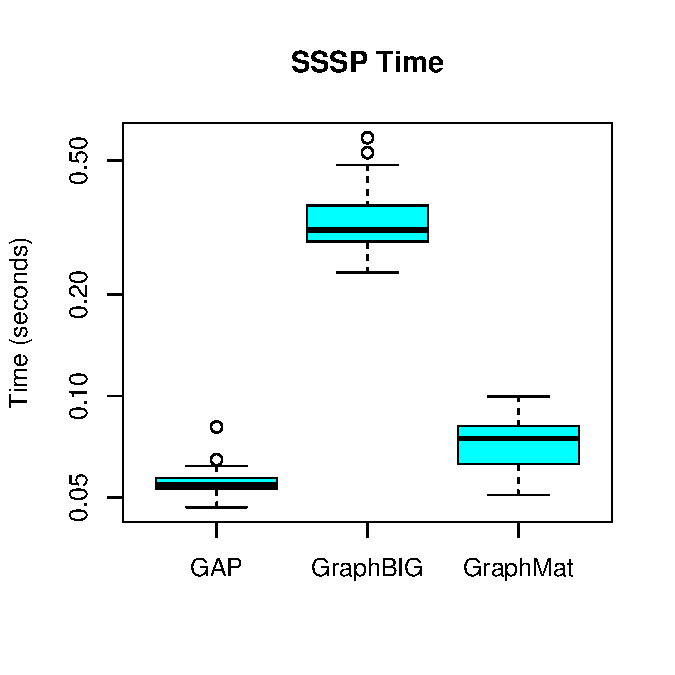
\includegraphics[width=0.6\columnwidth, trim=0 36pt 18pt 0, clip]{graphics/sssp_time.pdf}
	\caption{The $y$-axis is logarithmic.}
	\label{fig:sssp-time}
\end{figure}

\begin{figure}
	\centering
	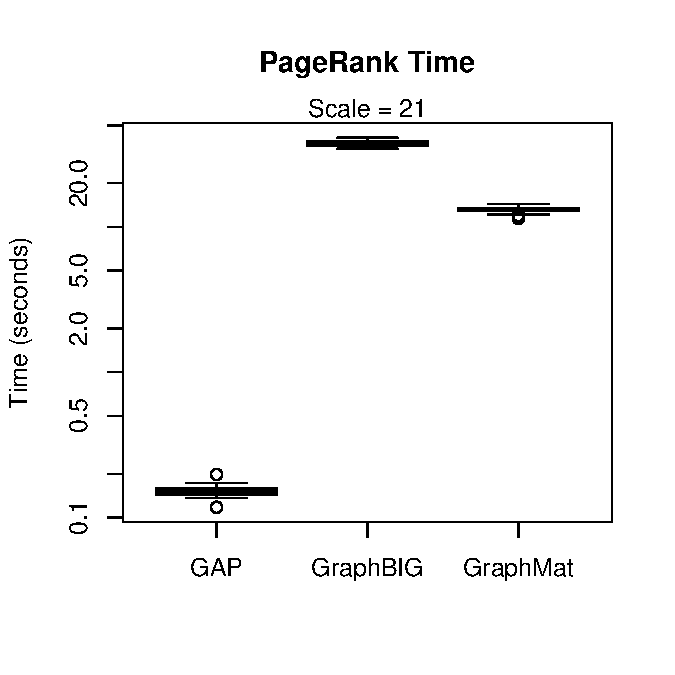
\includegraphics[width=0.6\columnwidth, trim=0 36pt 18pt 0, clip]{graphics/pr_time.pdf}
	\caption{The $y$-axis is logarithmic. GraphMat continues to run until none of the vertices' ranks change. [There is only one data point]}
	\label{fig:pr-time}
\end{figure}

\begin{figure}
	\centering
	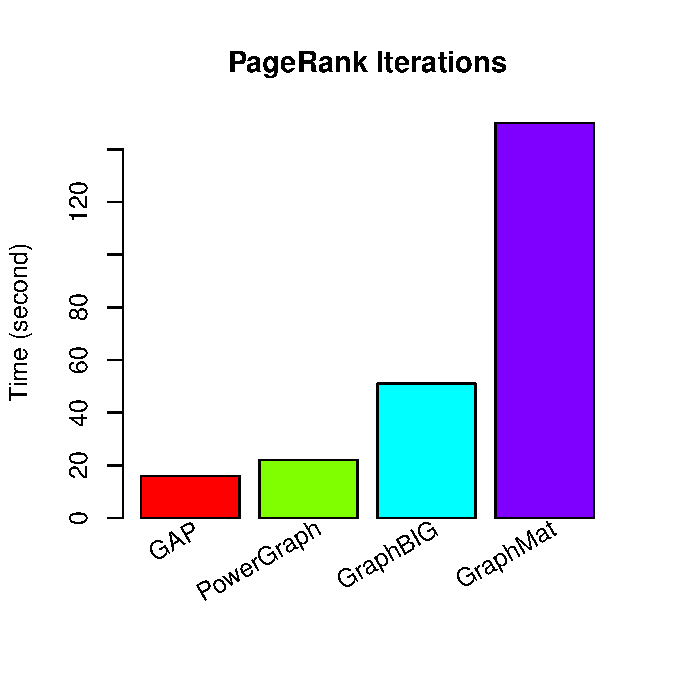
\includegraphics[width=0.6\columnwidth, trim=0 36pt 18pt 0, clip]{graphics/pr_iters.pdf}
	\caption{The $y$-axis \emph{not} logarithmic. GraphMat iterations are measured differently because of the ``think like a vertex'' paradigm and runs until none of the vertices' ranks change.}
	\label{fig:pr-iters}
\end{figure}
[Note that for figure Fig.\ref{fig:pr-iters}, mention time per iteration]

[Compare lines of code for implementation]

\begin{figure}
	\centering
	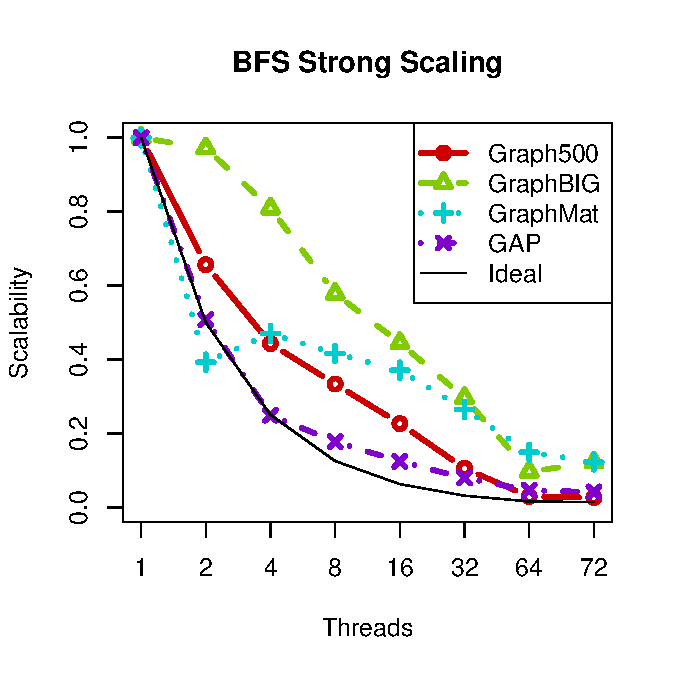
\includegraphics[width=0.8\columnwidth, trim=0 36pt 18pt 0, clip]{graphics/bfs_ss.pdf}
	\caption{Strong Scaling for $2^{20}$ vertices and an average of 16 edges per vertex.}
	\label{fig:bfs-ss}
\end{figure}

\begin{figure}
	\centering
	% trim left bottom right top
	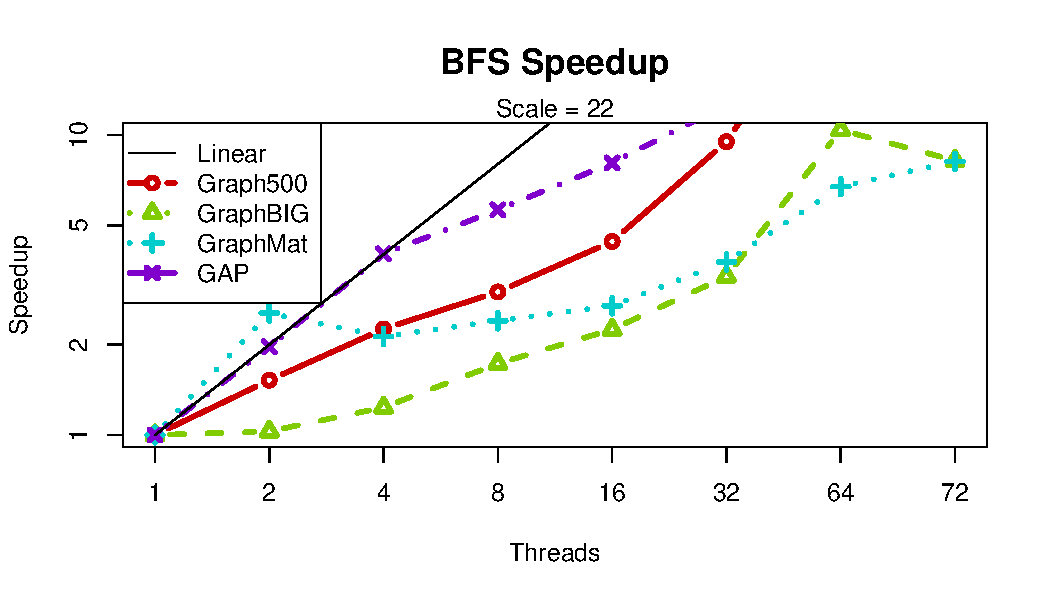
\includegraphics[width=\columnwidth, trim=0 36pt 18pt 0, clip]{graphics/bfs_speedup.pdf}
	\caption{Speedup.}
	\label{fig:bfs-speedup}
\end{figure}

%\section{Graph Processing Taxonomy}
%This is in the spirit of \cite{Doekemeijer:2015:GPFSurvey}. Here, ``|'' means ``or'' and ``+'' means ``and.'' FOSS means Free and Open Source Software. The quotes around ``yes'' for HPC mean that the product claims to be amenable to high performance computing. Whether these actually achieve their goal is one of the purposes of this project.
%\begin{table*}[t]
%	\begin{minipage}{\linewidth} % So the footnotes all get printed on the same page
%		\centering
%		%\small
%		\pgfplotstabletypeset[
%			col sep=comma,
%			string type, % Makes the .style={string type} redundant
%			columns={Name,Type,Parallelism,Target,FOSS,Source,Notes},
%			every head row/.style={after row=\midrule},
%			columns/Name/.style={string type, column type={l|}},
%			columns/Type/.style={string type},
%			% columns/HPC/.style={string type},
%			columns/Parallelism/.style={string type},
%%			columns/Comm./.style={%
%%				string type,
%%				postproc cell content/.style={%
%%					@cell content/.add={\footnotesize}
%%				}
%%			},
%			columns/Target/.style={string type},
%			columns/FOSS/.style={string type},
%			columns/Source/.style={string type},
%			columns/Notes/.style={
%				preproc cell content/.style={@cell content=
%					\ifx&##1&% Only make a footnote if the cell is nonempty
%						##1
%					\else
%						\footnote{##1}
%					\fi}
%			},
%		]{../report/platforms.csv}
%		\caption{Tools used for graph processing}
%		\label{tab:frameworks}
%	\end{minipage}
%\end{table*}


\section{Conclusion} % Begin with the end in mind...

\bibliographystyle{splncs03}
\bibliography{../drp}
\end{document}
